\section{Chemins dans l'arbre des fichiers.}
\textsl{Dans la suite j'emploie le mot directory ou le mot répertoire pour
désigner la même chose.}


Il y a plusieurs moyens de définir des chemins. On rappelle que la
racine de l'arbre est désignée par \com{/}.


\begin{enumerate}
  \item Chemin absolu en partant de la racine; exemple:
    \com{/etc/firefox/pref}
    
    Ce qui peut se lire de droite à gauche:  \com{pref} est dans le
    répertoire \com{firefox} et \com{firefox} est dans le répertoire
    \com{etc}, qui est à la racine\footnote{Noter que dans
      \com{/etc/firefox/pref}, \com{pref} peut être un répertoire ou
      un fichier, mais si je tape \com{/etc/firefox/pref/}, alors
      \com{pref} est obligatoirement un répertoire.}, ou bien de
    gauche à droite: \com{etc} est à la racine, \com{firefox} est dans
    \com{etc} et \com{pref} est dans le répertoire \com{firefox}.

    
    
  \item Chemins relatifs:  le point \com{.} désignant le répertoire
    courant, les deux points \com{..} désignant le 
    répertoire père et \com{\textasciitilde} ~ (tilde) désignant le
    \textsl{home directory}, 
    on peut définir des chemins \textsl{relatifs} (au-dessus,
    à coté, etc.), comme par exemple \com{../truc}.
\end{enumerate}
    
%\subsection{Se promener dans l'arbre des fichiers.}
On rappelle les deux  commandes \com{pwd} et \com{cd}:
\begin{itemize}
\item  \com{pwd} (print working directory): vous dit où vous êtes.
\item  \com{cd} pour changer de répertoire (change directory):
  
  \com{cd} sans argument vous ramène à votre home-directory. Sinon, la
  commande doit être

  \comc{cd}{chemin}

  où \comc{}{chemin} est un
  chemin, relatif ou absolu; exemple:

  \com{cd /usr/local/bin} (chemin absolu: on décrit le chemin depuis
  la racine),

  ou bien

  \com{cd ../truc/toto} (c'est à dire aller dans le répertoire père
  puis là, aller 
  dans \texttt{truc} puis  dans \texttt{toto} --qui doivent exister
  pour que ça fonctionne--): c'est un chemin relatif (on décrit le
  chemin depuis là où on est).

  Illustration (déplacement avec un chemin relatif): 

  \begin{center}
  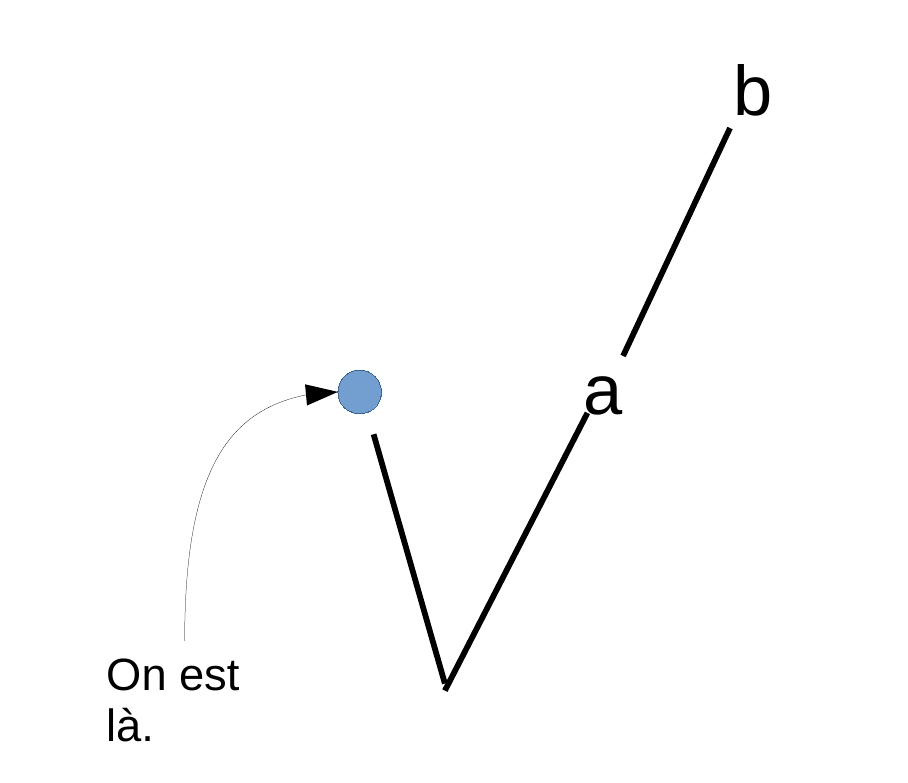
\includegraphics[width=0.25\linewidth]{images/mv.png}
  
  Après \com{cd ../a/b}, on est en b. 
  
  \end{center}
  
\end{itemize}

\subsubsection*{\exos}
à faire depuis un terminal\footnote{on dira plutôt \og shell\fg{} que
  terminal, c'est plus chic.}.
\begin{enumerate}
  \item Déplacements absolus et relatifs:
      \begin{itemize}
      \item aller directement dans \com{/etc/network}
      \item de là, aller dans \com{/etc}
      \item revenir dans le home directory.
      \end{itemize}
      (Note: vous avez certainement du faire un déplacement relatif).
    \item \`A quoi correspond: \com{cd ../..}?
\end{enumerate}
\section{La commande \ttt{ls}}
Regarder et jouer avec la commande  \com{ls} permet de se familiariser
avec les autres commandes qui fonctionnent toutes sur le même
principe:
\begin{enumerate}
\item \com{ls}

  sans option (\exx{tester}).
\item \comc{ls}{chemin}

  par exemple:

  \com{ls /usr/bin}

  \exo{} jouer avec
  différents types de chemins utilisés ci-dessus.
  
\item \com{ls} avec  options. Les options
  commencent par \com{-} (c'est le tiret, c'est à dire le signe
  \textsl{``moins''} du 6). 
  \begin{itemize}
  \item Placez vous d'abord  dans le home directory, puis tapez:

    \com{ls -a}

    Avec l'option \com{-a} \texttt{ls} montre les
      fichiers et répertoires cachés (installés par vos applications,
      leur nom commence par un point) \exx{(tester).}
    \item Avec l'option \com{-l}:

      \com{ls -l}

      on obtient  plein de renseignements (on verra
      ça plus tard) \exx{(tester).} 
    \item Combiner plusieurs options

      \com{ls -al}

      et puis aussi
      \com{ls -alt}

      (résultats triés par dates) et on peut aussi
      inverser l'ordre de tri:

      \com{ls -altr} \exx{(tester).}
    \item  Appliquer cette commande avec des options à un chemin:
      
      \com{ls -alt /var/log}

      etc, etc. \exx{(tester).}
  \end{itemize}

  Noter que la syntaxe des options est assez souple: elles peuvent
  être mises dans n'importe quel ordre; de plus  au lieu de \com{ls -alt
    /var/log} on aurait pu écrire

  \com{ls -l -a -t /var/log}
  
  mais en ne voit pas trop quel en aurait été l'intérêt.
\end{enumerate}

\section{Quelques autres commandes}
\begin{itemize}
\item Les systèmes Unix contiennent leur documentation (manual). La
  commande est \com{man}.

  \exo{} jouer avec \com{man} par exemple:

  \com{man ls}

  ou bien:
  \com{man man}

   Le résultat peut être indigeste!
\item \com{whoami}

  Vous donne votre \textsl{login}. En principe votre home-directory
  est \texttt{/home/}$+$le résultat de cette commande. \exx{Le vérifier}.
  
\item \com{less} permet de voir un fichier page par page (appuyer sur
  espace pour aller à la page suivante). On peut aussi sauter à la
  prochaine occurrence d'un motif (taper \textsf{/motif} quand on est
  dans less). (\textsf{q pour
    quitter less}). Un exemple \exx{(tester)}:

  \com{less /etc/services}
\end{itemize}

%et des commandes inévitables:
\begin{itemize}
\item \comc{rm}{chemin}

  Efface un fichier (celui qui est au bout du chemin). 
  \small{\textdbend}  \textbf{ Attention, on travaille sans 
    filet! Quand un fichier est effacé, on n'a plus qu'à aller
    chercher la sauvegarde (si on en a une).}

  Exemples:
  
  \com{rm toto}
  
  \com{rm \textasciitilde/truc/machin/toto} 
  
 \item   \comc{mkdir}{chemin}

   Crée un répertoire (il ne doit pas déjà exister). Exemples:

   \com{mkdir MonDir}

   \com{mkdir /truc/machin/chose}

   Ça fonctionnera seulement si  /truc/machin/ existe déjà. Sinon
   faire:
   
   \com{mkdir -p /truc/machin/chose}

   et on crée comme ça tous les répertoires.
 \item \comc{rmdir}{chemin}

   Efface un répertoire \red{vide}. Exemple:

   \com{rmdir \textasciitilde/truc/machin/chose}

   Et si le répertoire n'est pas vide? On a un message d'erreur. Alors
   il faut utiliser la 
   commande \com{rm} avec l'option \com{-r} (récursive) qui efface le
   répertoire et tout ce qu'il contient:

   \com{rm -r \textasciitilde/truc/machin/chose}

   Si on a peur, on peut ajouter \com{-i}, qui vous demandera de
   confirmer chaque effacement:

   \com{rm -ri \textasciitilde/truc/machin/chose}

 \item Filtre: \com{grep}

   \com{grep udp /etc/services}  va lister toutes les lignes qui
   contiennent \texttt{udp} dans le fichier \texttt{/etc/services}.

   \com{grep -v udp /etc/services}  va lister toutes les lignes qui ne
   contiennent \underline{\textbf{\large pas}} \texttt{udp}.

   Si on rajoute \com{-i} (par exemple \com{grep -v nagios
     /etc/services}) la recherche ne tient plus compte de la casse
   (minuscules ou majuscules).

\end{itemize}
\exo{}

La commande:

\com{touch toto}

crée un fichier vide de nom \com{toto}.

Créer des répertoires (emboîtés), créer des fichiers vides dedans et
tout effacer\footnote{Mettez donc l'option \com{-i} quand vous
  utilisez \com{rm}.}. 

\section{Plomberie}
Deux définitions:
\begin{enumerate}
  \item \textbf{Entrée standard:} ce que les commandes lisent. Par défaut, c'est
    votre clavier.
  \item \textbf{Sortie standard:} là où les commandes écrivent: la fenêtre
    courante par défaut.
\end{enumerate}

Alors:
\begin{itemize}
\item On peut rediriger la \textbf{sortie standard} vers un fichier:

\com{ls /var/log >toto}

Les résultats vont dans \com{toto} plutôt que sur l'écran. Regarder
ensuite le fichier \com{toto} avec:

\com{less toto}

\item Avec \com{<} c'est l'entrée standard qu'on redirige depuis un
  fichier (on verra ça plus tard).

\item Le \og pipe\fg{}:

  Le principe est le suivant: étant donné des
  commandes \com{A} et \com{B}, on fait en sorte que la sortie standard
  de  \com{A} soit l'entrée standard de \com{B}:

  \com{A|B}

  (le caractère \com{|} est obtenu par \texttt{Alt~Gr} et la touche ``6'').
  
  \exx{Exemple (à tester):}

  \begin{itemize}
  \item On commence par  \com{grep tcp /etc/services}

    qui liste les lignes qui contiennent \texttt{tcp} dans
    \texttt{/etc/services}. Évidemment, le résultat sort sur l'écran
    (la sortie standard).
    
  \item La commande \com{grep}, s'il n'y a pas de chemin défini, 
    lit sur l'entrée standard.

    Donc

    \com{grep tcp /etc/services | grep Protocol}

    va:
    \begin{enumerate}
      \item Filtrer les lignes de \com{/etc/services} qui contiennent
        \texttt{tcp}.
      \item Ensuite, \com{grep Protocol} récupère ce qui normalement
        va sur l'écran et filtre les lignes qui contiennent
        \texttt{Protocol}.
    \end{enumerate}
    et voilà. On peut chaîner autant de commandes qu'on veut. Par
    exemple, la commande:

    \comc{nl}{chemin vers un fichier}
    
    numérote les lignes d'un
    fichier (regarder par exemple ce que donne \com{nl
      /etc/services}); en l'absence d'argument, la commande \com{nl}
    lit l'entrée standard.

    On peut donc chaîner 3 commandes (\com{grep}, \com{grep} et \com{nl}):
    
    \com{grep tcp /etc/services | grep Protocol|nl}

    et \textbf{compter} ainsi le nombre de lignes du fichier
    \com{/etc/services} qui contiennent \texttt{tcp} \textbf{et}
    \texttt{Protocol}.

    Et puis on peut finir par la commande \com{tail}; ainsi

    \com{tail /etc/services}

   lit le fichier \texttt{/etc/services} et en montre la fin, mais
   \com{tail} sans chemin vers un fichier 
      lit sur l'entrée standard. Donc, pour savoir combien de lignes
      dans \texttt{/etc/services} contiennent \texttt{tcp} et
      \texttt{Protocol}, et pour limiter le nombre de lignes qui, à la
      fin, sortent sur l'écran, on
    peut taper (4 commandes chaînées):



    \com{grep tcp /etc/services|grep Protocol|nl|tail}\footnote{ou
      \com{grep tcp /etc/services|grep Protocol|nl|tail -1} cf. \com{man tail}}
    
  \end{itemize}
\end{itemize}
\section{Quelques petits trucs à savoir à propos du shell}
Le shell, c'est le programme qui interprète vos commandes. En fait, il
existe plusieurs shells disponibles, mais le plus populaire est celui
de \textsf{Steve 
Bourne}, qui a connu plusieurs évolutions, et qui s'appelle maintenant
\og \textsf{Bourne Again Shell}\footnote{ah, ah, l'astuce!}\fg{}, soit
\com{bash}. Si 
vous tapez:

\com{which bash}

vous verrez où il est installé (\com{which} vous donne le chemin vers
une commande).

Il existe d'autres shells, comme \com{zsh}, mais bon...

Des trucs bien pratiques à savoir:
\begin{itemize}
\item La complétion automatique:

  C'est plutôt puissant. On utilise le caractère \texttt{Tab}.

  Essayez:

  \exx{a\texttt{Tab}}  (deux caractères: le \exx{a} et le \exx{\texttt{Tab}}),

  puis:

  \exx{ap\texttt{Tab}} (note: il faut parfois taper 2 fois
  \texttt{Tab}).

  On voit toutes les commandes accessibles qui commencent par
  \texttt{ap}.

  De plus, certains logiciels introduisent des règles de
  complétion. Par exemple:

  \com{evince toto.\texttt{Tab}}

  proposera de visualiser le fichier \texttt{toto.pdf}
    s'il existe.
  \item L'historique:
    \begin{itemize}
      \item à titre d'exemple, \com{!evin} relance la dernière
        commande qui commençait 
        par \com{evin} (attention, tout de même: pensez aux dégats
        possible de \com{!rm}). 
      \item \com{history} donne l'historique des commandes, numéroté.
        On peut par exemple relancer la 135\ieme commande en tapant:

        \com{!135}

        cet historique persiste, même si vous redémarrez la machine.

        On peut aussi se servir des flèches pour naviguer dans
        l'historique.

        Un bon conseil: \exx{testez, retestez!}
        

    \end{itemize}
\end{itemize}

